\chapter{Технологическая часть}
Вариант 4 лабораторной работы заключается в реализации алгоритма поиска подстроки в строки КМП, используя параллельные вычисления. Для домашнего задания выбран алгоритм получения массива lps (longest prefix suffix). При выполнении дошанего задания использовался язык программирования C++. Необходимо реализовать граф управления программы, информационный граф программы, операционную историю программы, информационную историю программы. 
\section{Исходный код программы}
На листинке \ref{lst:kmp} приведен код программы, которая формирует матрицу без i-й строки и j-го столбца. 
\begin{lstinputlisting}[
	caption={Заполнение массива lps},
	label={lst:kmp},
	linerange={4-29}
	]{../src/main/Algo.cpp}
\end{lstinputlisting}
\section{Модели графов}
Вершины А и В связываются операционным отношением, если вершина В может быть выполнена сразу после А. Вершины А и В связаны информационным отношением, если вершина В использует результат работы вершины А. Для операционного графа вершинами являются операторы, а дугами операционные отношения. Для информационного графа вершинами являются операторы, а дугами информационные отношения. Для графа операционной истории вершинами является срабатывание операторов, а дугами операционные отношения. Для графа информационной истории вершинами являются срабатывания операторов, а дугами информационные отношения.
На рисунках \ref{fig:gy}--\ref{fig:ii} представлены граф управления программы, информационный граф программы, операционная история программы, информационная история программы.

\begin{figure}[h]
	\centering
    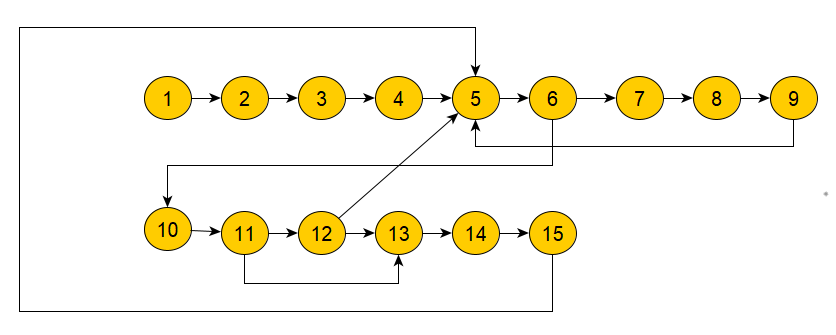
\includegraphics[height=0.20\textheight]{img/GY.png}
    \caption{Граф управления программы}
    \label{fig:gy}
\end{figure}
\begin{figure}[h]
	\centering
	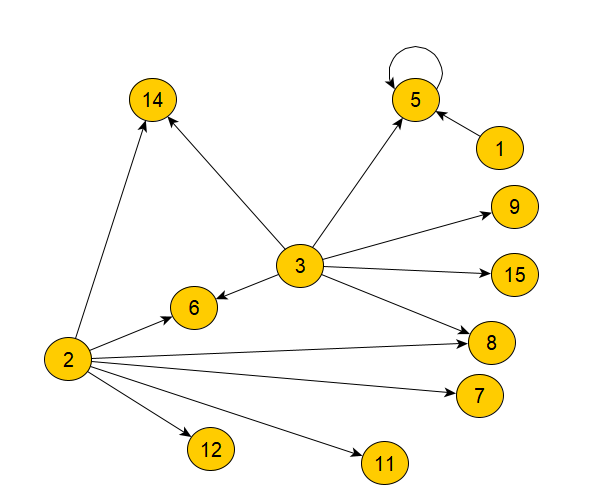
\includegraphics[height=0.4\textheight]{img/IG.png}
	\caption{Информационный граф программы}
    \label{fig:ig}
\end{figure}
\begin{figure}[h]
	\centering
	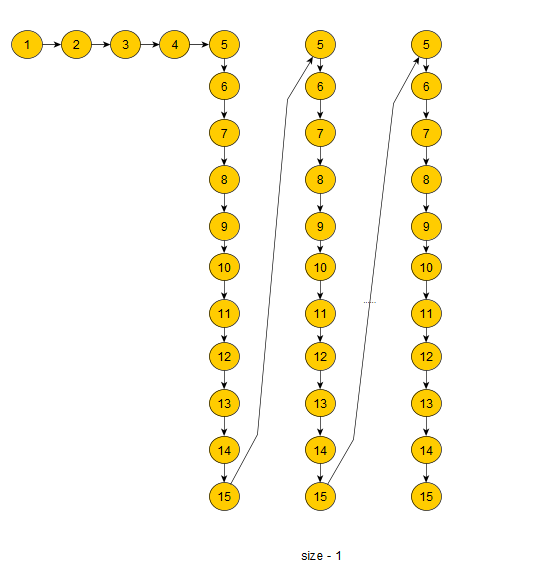
\includegraphics[height=0.5\textheight]{img/OI.png}
	\caption{Операционная история программы}
	\label{fig:oi}
\end{figure}
\begin{figure}[h]
	\centering
	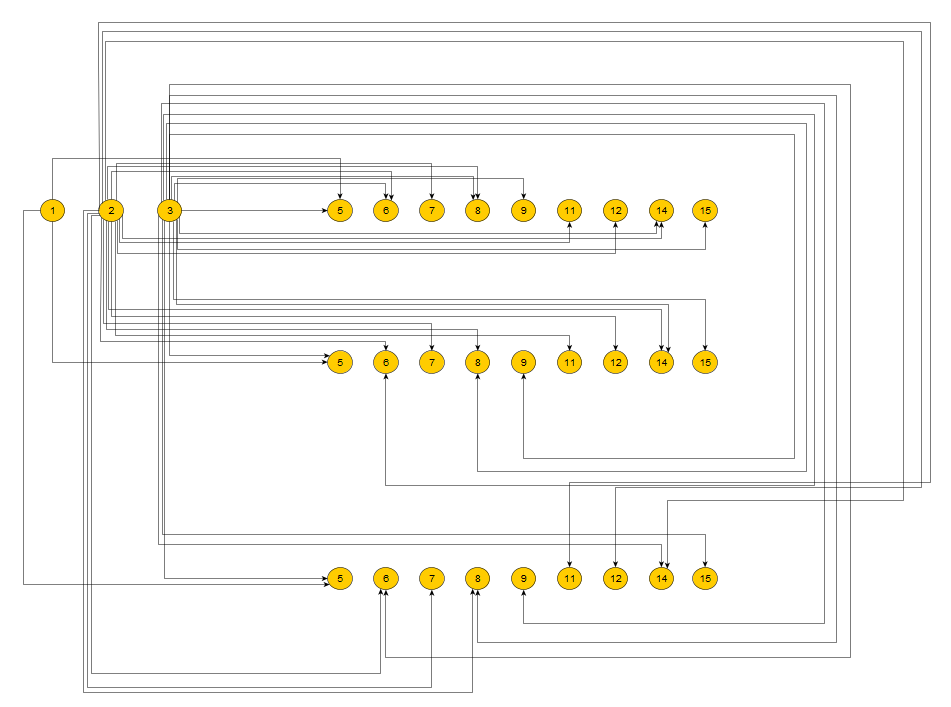
\includegraphics[height=0.45\textheight]{img/II.png}
	\caption{Информационная история}
	\label{fig:ii}
\end{figure}
\clearpage

